\chapter{Processos}

\begin{definicao}{Processo}
  É um programa em execução, composto por:
  \begin{itemize}
    \item Código em execução;
    \item Pilha de execução e seu apontador;
    \item Contado de programa (\texttt{PC});
    \item Valores de registradores de máquina;
    \item E outras informações.
  \end{itemize}
\end{definicao}

Cada processo possui um identificador único, conhecido como \textit{pid}. As informações do processo ficam armazenadas na \textbf{tabela de processos}, sendo o \textit{pid} seu indexador na tabela.

Durante a execução, o processo compartilha o processador com outros processos, sendo eles escalonados ao longo do tempo. A interação entre processos ocorre por mecanismos de comunicação próprios.

Por fim, existem dois escopos que carregam variáveis sobre a execução do processo:

\begin{itemize}
  \item \textbf{Ambiente:} contendo o espaço de endereçamento, arquivos abertos, processos filhos, sinais, estatísticas de uso, etc.;

  \item \textbf{Execução:} contendo registradores utilizados pelo processo, como o PC e o apontador de pilha, e o estado de execução do processo.
\end{itemize}

\begin{figure}
  \centering
  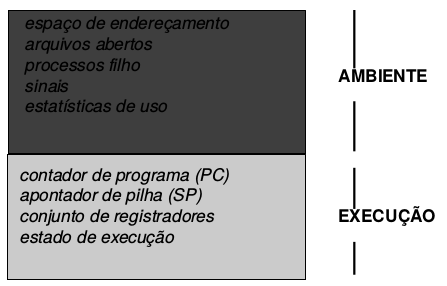
\includegraphics[width=.5\textwidth]{process-model}
  \caption{Modelo padrão de escopo de um processo}
  \label{fig:process-model}
\end{figure}
















\section{Modelo de Processos}
Classificamos os processos em relação ao custo de troca de contexto e manutenção:

\begin{itemize}
  \item \textbf{\textit{Heavyweight}:} são os processos tradicionais. Na sua entrada da tabela de processos temos tanto as informações de ambiente como as de execução;
  \item \textbf{\textit{Lightweight}:} são as \textit{threads}. Sua entrada na tabela de processos só contém informações de execução.
\end{itemize}

No modelo \textit{heavyweight}, também chamado de modelo tradicional, cada processo tem um único fluxo de controle, ou seja, em um dado momento ele só tem um valor de \texttt{PC}. Este processo roda independente dos demais e pode conter processos \textit{threads} que dependem dele.

Todo sistema operacional deve possuir mecanismos que permitam a criação de processos. Geralmente, um processo somente é criado por outro processo, o que nos leva uma \textbf{hierarquia de árvore de processos} (Figura \ref{fig:process-tree}). Entretanto, é necessário frisar que a árvore de processos não é de fato implementada. A partir do campo de ID do processo pai (PPID), podemos virtualmente implementar essa árvore. Implementá-la de fato seria muito custoso.

\begin{figure}[h]
  \centering
  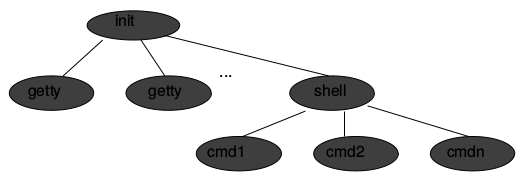
\includegraphics[width=0.6\textwidth]{process-tree}
  \caption{Esquema de uma árvore de processos padrão}
  \label{fig:process-tree}
\end{figure}




















\section{Estado do Processo}
Apesar de processos serem relativamente auto-suficientes, muitas vezes eles necessitam de acessar outros recursos (discos, terminais) ou mesmo se comunicar com outros processos. Quando um processo está ocioso, esperando que um evento aconteça, nós dizemos que ele está bloqueado. Em algumas situações, o processo pode ser bloqueado a revelia pelo sistema operacional. Podemos ter os seguintes estados:

Estados:
\begin{itemize}
  \item \textbf{Rodando:} processo em execução
  \item \textbf{Bloqueado:} processo parado, aguardando alguma coisa;
  \item \textbf{Pronto:} processo parado, pronto para ser executado, aguardando sua vez.
\end{itemize}

Usando a Figura \ref{fig:proc-states} como referências, podemos ilustrar as diversas passagens de estados ao longo da vida de um processo:

\begin{enumerate}
  \item O processo bloqueia-se à espera de um evento ou recurso;

  \item O evento ou recurso esperado pelo processo está disponível.Ele agora pode se executar, passando para o estado de \textit{Pronto};

  \item O processo é escolhido pelo escalonador para execução;

  \item O tempo de posse do processador pelo processo acabou. O SO retira o processador do processo.
\end{enumerate}

\begin{figure}[ht]
  \centering
  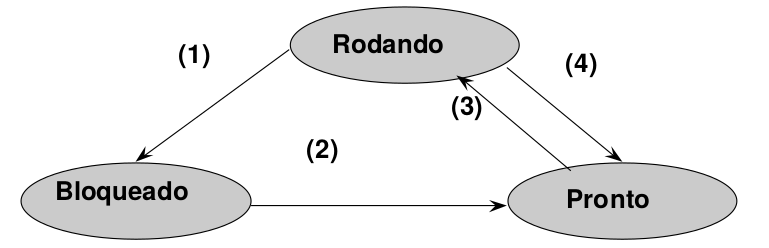
\includegraphics[width=.75\textwidth]{proc-states}
  \caption{Possíveis estados de um processo.}
  \label{fig:proc-states}
\end{figure}

















\section{Tabela de Processos}
\begin{definicao}{Tabela de Processos}
  Estrutura que contem os todas as informções relativas à manutenção de cada processo do SO, guardando os campos de gerência de processos, memória e arquivos. Possui uma entrada para cada processo.
\end{definicao}

Em relação a \textbf{gerência de processos}, as informações guardadas normalmente são: \textit{pid}, valor dos registradores de execução e PC, valor da palavra de estado, valor do apontador de pilha, estado do processo, instante do início do processo, tempo de processador utilizado e outros.

Em relação a \textbf{gerência de memória}, são guardados o endereço do segmento de texto, dados e pilha, sendo estes mandatórios. Podemos ter também estado da saída, informações sobre proteção e outros. Note que o segmento de texto é a porção de código do processo, que normalmente é \textit{read only}. Alguns sistemas com área de memória pequena tornam essa área \textit{read-write}, para uso eficiênte da memória, porém essa estratégia oferece riscos de segurança.

Em relação a \textbf{gerência de arquivos}, são guardados o diretório raíz e de trabalho, descritores de arquivos abertos, parâmetros de chamadas em andamentos e outras.




\subsection{Troca de Contexto}
\begin{definicao}{Contexto}
  No que diz respeito a processos, o contexto será o conjunto de valores dos registradores do processo.
\end{definicao}

Dessa forma, define-se a troca de contexto como a operação de salvamento dos registradores de um processo, para restauração dos conjunto de registradores de outro processo. Tal operação permite que haja a efetiva troca de processos no processador.




















\section{Escalonamento de Processos}
O algoritmo de escalonamento de processos é o responsável pela determinação de que processo, dentro do conjunto de processos prontos, vai rodar e por quanto tempo. Quando um processo solicita operações blocantes, sua execução fica suspensa até que o evento solicitado ocorra.

\textbf{Nota:} podemos citar como operações blocantes requisições ao disco, memória, entrada e saída, entre outras.

Para garantir um bom algoritmo de escalonamento, alguns \textbf{critérios} devem ser seguidos:
\begin{itemize}
  \item \textbf{\textit{Fairness}:} garantir que todos os processos do sistema terão chances de uso do processador, ou seja, \textbf{não há \textit{starvation}}. Garantir que os processos tenham chances \textit{iguais}, é algo muito forte e não usamos essa definição;

  \item \textbf{Eficiência:} se há demanda, a CPU deve estar ocupada;

  \item \textbf{Minimizar o tempo de resposta:} o tempo total decorrido até que um processo produza uma resposta ao usuário/sistema;

  \item \textbf{Minimizar o \textit{waiting time}:} ou seja, o tempo de resposta entre os estados \textit{Ready} e \textit{Running};

  \item \textbf{Maximizar o \textit{thoughtput}:} aumentar o número de processos conclúidos em um determinado tempo.
\end{itemize}

\begin{definicao}{Preempção}
  Suspensão temporária da execução de um processo.
\end{definicao}

Podemos classificar escalonadores segundo sua preempção:

\begin{itemize}
  \item \textbf{Escalonadores não-preemptivos:} quando um processo obtém o processador, ele roda até o seu fim ou até que ele peça uma operação blocante.

  Isto simplifica o projeto do escalonador, porém permite que o processo detenha a CPU por tempo arbitrário, levando-o ao monopólio do processador. Isto acaba por violar todos os critérios de um bom escalonador;

  \item \textbf{Escalonadores preemptivos:} cada processo possui um tempo máximo de permanência, chamado \textbf{\textit{quantum}}, de posse do processador. Quando o \textit{quantum} termina, o SO retira o processador deste processo, para permitir a execução de outro processo.

  Desta forma, estes escalonadores garantem um uso mais balanceado da CPU, o que levam a eles serem usados na maioria dos SOs. Entretanto, seu projeto é consideravelmente mais complexo, uma vez que os processos devem proteger suas regiões críticas de outros processos concorrentes.
\end{itemize}

\begin{definicao}{Região Crítica}
  Área que contém as estrutura de dados importantes de um processo em execução, não podendo ser acessada por concorrentemente, mas sim atômicamente.
\end{definicao}

O tempo de execução do processo é controlado por um \textit{clock} que gera interrupções em uma determinada frequência, chamadas de \textit{clock tick}. Tal ferramenta está presente em qualquer processador moderno.

O SO mantem um contador que é decrementado a cada \textit{clock tick}. Quando este contador chega a zero, o tempo de permanência do processo acabou e ele será retirado do processador. O valor inicial deste contador corresponde ao tempo máximo de permanência do processo com a CPU, denominado, \textbf{\textit{time slice}}.

Dado isto, podemos listar as \textbf{políticas de algoritmos de escalonamento} existentes.



\subsection{\textit{First Come First Served}}
Os processos que solicitam a CPU são colocados em uma fila \textit{ready}, gerênciada segundo a política FCFS: o primeiro processo que entrar, será o primeiro a ser executado por completo. Desta forma, é importante notar que este algoritmo é \textbf{não-preemptivo}.

\begin{figure}
  \centering
  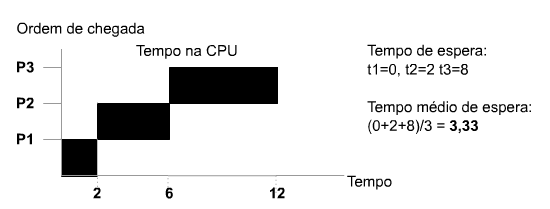
\includegraphics[width=0.75\textwidth]{scale-fcfs}
  \caption{Execução de processos em política FSFC com ordem chegada P1, P2 e P3.}
  \label{fig:scale-fcfs}
\end{figure}





\subsection{\textit{Round Robin}}
Cada processo tem o direito de usar o processador por um intervalo de tempo pré-definido, denominado \textbf{\textit{quantum}}. Quando este intervalo se esgota, o processador é dado a outro processo e o processo retirado vai para o fim da fila de processos. É versão preemptiva da política FSFC, sendo um algoritmo justo.

\begin{figure*}[h]
  \begin{subfigure}[t]{0.45\textwidth}
    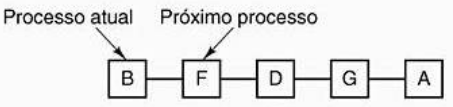
\includegraphics[width=0.9\textwidth]{round-robin-1}
    \caption{Fila de processos em $t_1$}
    \label{fig:round-robin-1}
  \end{subfigure}
  ~
  \begin{subfigure}[t]{0.45\textwidth}
    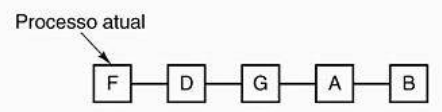
\includegraphics[width=0.9\textwidth]{round-robin-2}
    \caption{Fila de processos em $t_2$, ao fim do \textit{quantum} do processo $B$}
    \label{fig:round-robin-2}
  \end{subfigure}

  \caption{Escalonamento circular usando \textit{round robin}}
  \label{fig:round-robin}
\end{figure*}



\subsection{Escalonamento com Prioridades}
Baseia-se no fato de que alguns processos são prioritários e, assim, devem ser executados antes dos outros. A cada processo é atribuída uma prioridade e os que tem maior prioridade são executados primeiro.

A prioridade pode ser definida de duas formas:
\begin{itemize}
  \item \textbf{Estaticamente:} os processos são divididos em classes e a cada classe é atribuída uma prioridade. A cada prioridade, existe uma fila de prontos associada. A política nas filas pode ser arbitrária;

  \item \textbf{Dinâmicamente:} o sistema analisa o comportamento dos processose atribui prioridades favorecendo um certo tipo de comportamento. Por exemplo, processos com I/O podem ter prioridades altas. O cálculo da prioridade pode ser dado por $1/f$, onde $f$ é a fração do \textit{quantum} de tempo utilizado na última rodada do processo.
\end{itemize}

 Note que é possível que um processo pode monopolizar a CPU caso ele precise de muito tempo de processamento e sua prioridade for a maior de todas. A técnica de prioridade dinâmica tenta justamente mitigar este comportamento.

\begin{figure}[h]
  \centering
  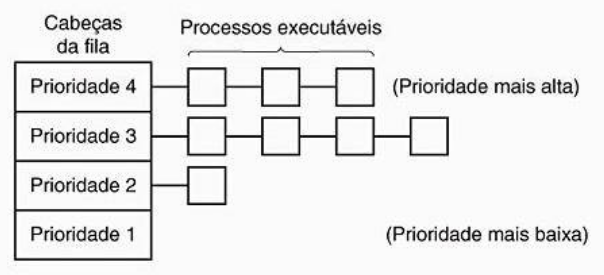
\includegraphics[width=0.75\textwidth]{priority-queue}
  \caption{Escalonamento com quatro categorias de prioridades}
  \label{fig:priority-queue}
\end{figure}




\subsection{\textit{Shortest Job First}}
Aqui, dado um conjunto de \textit{jobs} prontos, executamos os \textit{jobs} com menor tempo de execução antes.

Note que este algoritmo pode não ser muito justo, pois, supondo um processo com uma dada prioridade, este pode entrar em \textit{starvation} se todo novo processo que entrar na fila tiver tempo de execução menor que ele.

\begin{figure*}[h]
  \begin{subfigure}[t]{0.45\textwidth}
    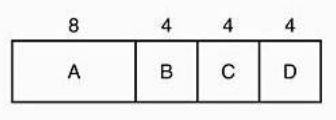
\includegraphics[width=0.9\textwidth]{sjf-1}
    \caption{Fila de processos crua}
    \label{fig:sjf-1}
  \end{subfigure}
  ~
  \begin{subfigure}[t]{0.45\textwidth}
    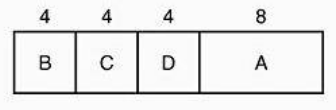
\includegraphics[width=0.9\textwidth]{sjf-2}
    \caption{Fila de processos organizada em SJF}
    \label{fig:sjf-2}
  \end{subfigure}

  \caption{Uso do \textit{shortest job first}}
  \label{fig:sjf}
\end{figure*}





















\section{\textit{Threads}}
\textit{Threads}, ou linhas de controle múltiplas, foram criadas visando maior concorrência na execução de processos. Nelas, o processo é dividido em dois: processo em si, correspondendo ao ambiente, e a \textit{thread}, correspondendo a execução.

Um processo pode ser composto por várias \textit{threads}, onde uma \textit{thread} pode se bloquear a espera de um recurso e outra, do mesmo processo ou não, pode se executar, paralelamente. A entidade que realmente executa é a \textit{thread}, sendo o processo apenas o ambiente.

\begin{figure}[h]
  \centering
  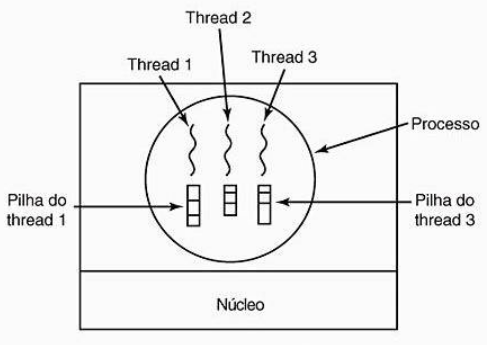
\includegraphics[width=.7\textwidth]{threads}
  \caption{Um processo com 3 \textit{threads}, cada uma com sua pilha de execução}
  \label{fig:threads}
\end{figure}

Aqui, \textbf{a troca de contexto é mais leve}, dado que esta troca entre \textit{threads} de um mesmo processo só diz respeito a execução e não ao ambiente. Frisamos que \textbf{\textit{threads} guardam apenas o contexto de execução e não de ambiente}.

Dado isto, estas \textit{threads} compartilham as mesmas variáveis globais, memória, descritores de arquivo e outros recursos. Logo, são necessários mecanismos de \textbf{sincronização} destes recursos: variáveis \textit{mutex} e variáveis de condição.

Podemos ter dois tipos de \textit{threads}:
\begin{itemize}
  \item \textbf{Estáticas:} o número de linhas de controle que irão compor o processo é definido em tempo de compilação, fazendo com que a execução comece com o número determinado;

  \item \textbf{Dinâmicas:} as \textit{threads} são criadas e destruidas dinâmicamente, ao longo da execução do processo, criadas com primitivas específicas. A execução começa com uma \textit{thread} apontando para o início da rotina \textit{main}. Esta técnica é a mais comum.
\end{itemize}






\subsection{Implementação}
É possível implementar \textit{threads} de duas maneiras. A primeira é a \textbf{nível de \textit{kernel}}. Aqui, as abstrações de processo e \textit{threads} são implementadas pelo sistema operacional, de maneira protegida. Logo, existe a tabela de processos e uma tabela de \textit{thread} para cada processo. Isto garante um alto grau de concorrência, porém o custo da troca de contexto entre \textit{threads} continua alto, pois esta gera trocas de contexto entre modo protegido e usuário, o que é um \textit{overhead} custoso.

A segunda forma é a implementação a \textbf{nível de usuário}, simulando as \textit{threads} através de bibliotecas. Dessa forma, o custo da troca de contexto é baixo, porém quando uma \textit{thread} realizar uma operação blocante, o seu processo inteiro será bloqueado e, consequentemente, todas as suas \textit{threads-irmãs}.







\section{\textit{Deadlock}}
\begin{definicao}{\textit{Deadlock}}
  Um conjunto de processos está em \textit{deadlock} se cada processo pertencente ao conjunto estiver esperando por um evento que somente um outro processo pertencente ao mesmo conjunto pode fazer ocorrer. Como todos estão ocupados, nenhum pode provocar a ocorrência de eventos. Logo, \textbf{é uma espera eterna por recursos}.
\end{definicao}

\begin{figure}[ht]
  \centering
  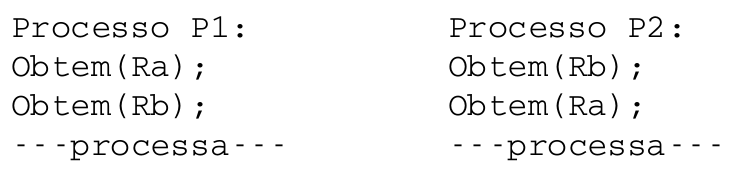
\includegraphics[width=0.7\textwidth]{deadlock}
  \caption{Uma situação clássica de \textit{deadlock}. P1 obtém \texttt{Ra}, e logo pede \texttt{Rb}. Entretanto, \texttt{Rb} está sob posse de P2, logo P1 bloqueia. Por sua vez, P2 está bloqueado, aguardando \texttt{Ra}. Logo, ambos estão bloqueados, aguardando recursos ocupados}
  \label{fig:deadlock}
\end{figure}

\begin{definicao}{\textit{Livelock}}
  Ocorre quando um conjunto de processos tentam acessar um recurso por meio de \textit{polling}, sempre encontrando esse recurso ocupado, pois estes estão alocados a processos que fazem parte do mesmo conjunto. Dessa forma, estes processos bloqueiam-se mutuamente. Logo, \textbf{há uma espera circular dentro do conjunto de processos}.
\end{definicao}

\begin{definicao}{\textit{Polling}}
  Técnica onde verifica-se periodicamente o estado de um recurso.
\end{definicao}

\begin{figure}[ht]
  \centering
  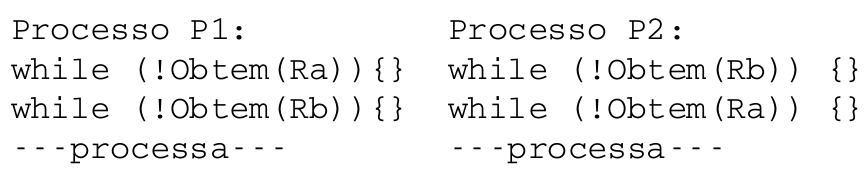
\includegraphics[width=0.7\textwidth]{livelock}
  \caption{Uma situação clássica de \textit{livelock}. A situação é análoga a da Figura \ref{fig:deadlock}, onde há um \textit{deadlock}. Entretanto, ao invés de se bloquear, os processos fazem \textit{polling} eterno.}
  \label{fig:livelock}
\end{figure}

\textbf{Nota:} Do ponto de vista teórico, \textit{livelock} e \textit{deadlock} tem significados equivalentes.

\begin{definicao}{\textit{Starvation}}
  Ocorre quando um conjunto de processos é indefinidamente preterido porque sua prioridade é menor que a prioridade de outros conjuntos de processos. Ou seja, é \textbf{uma espera por um tempo indefinido por recursos}.
\end{definicao}










\section{Comunicação entre Processos}
Processos interagem entre si, trocando informações, o que pode ser feito de duas formas: compartilhamento de variáveis ou troca de mensagens.


\subsection{Compartilhamento de Variáveis}
Nesta técnica, um processo escreve um valor em uma posição de memória e outro processo lê este mesmo valor.

Entretanto, a ordem e o tempo de execução dos processos não é previsível, dada a política de escalonamento do SO. Com isso, algumas incosistências podem ocorrer nestas áreas de memória compartilhadas, resultando em \textbf{condições de corrida}.

\begin{figure}
  \centering
  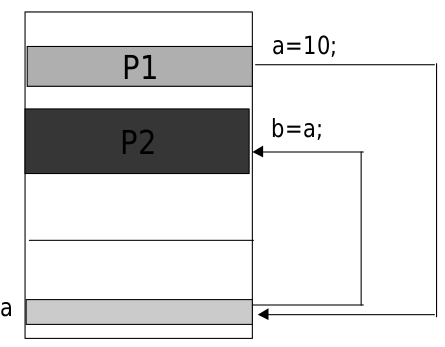
\includegraphics[width=0.5\textwidth]{variable-sharing}
  \caption{Processos $P1$ e $P2$ compartilhando a mesma posição $a$ de memória}
  \label{fig:variable-sharing}
\end{figure}

\begin{definicao}{Condição de Corrida}
  Quando dois ou mais processos acessam concorrentemente as mesmas posições de memória e o valor final contido nestas posições \textbf{depende da ordem} na qual os processos foram executados, então temos uma condição de corrida.
\end{definicao}

A condição de corrida pode não ser um erro ou algo indesejável. Alguns programadores podem tirar proveito disso. Além disso, podemos definir que os processos escrevam na mesma posição, porém forçando ser o mesmo valor. Neste último caso, \textit{não temos condição de corrida}. Porém, na maioria dos casos, é desejável eliminar as condições de corrida.





\subsection{Exclusão Mútua}
Garantir que processos ou \textit{threads} executem de forma ordenada, acessando seções críticas de maneira exclusiva é uma forma de garantir a \textbf{exclusão mútua}.

\begin{definicao}{Seção Crítica}
  Recurso ou parte do código protegida por mecanismos de exclusão mútua.
\end{definicao}

Para garantir uma exclusão mútua eficiente, a solução deve levar em contra os seguintes requisitos:
\begin{itemize}
  \item \textbf{Exclusão mútua:} a solução não pode permitir que dois processos acessem a seção crítica simultaneamente;

  \item \textbf{Progresso:} se a seção crítica está vazia e existem processos querendo acessá-la, apenas estes processos devem participar da decisão de quem vai acessá-la. Ou seja, \textbf{nenhum processo executando fora de sua seção crítica pode bloquear outros processos}.

  \item \textbf{Espera limitada:} deve existir um limite no número de vezes que outros processos acessam a seção crítica quando um processo está esperando por ela. Ou seja, \textbf{nenhum processo deve esperar eternamente para entrar em sua seção crítica}.
\end{itemize}

\textbf{Nota:} é importante frisar que levamos em conta que o programador seja correto em sua implementação, ou seja, que ele irá utilizar corretamente as ferramentas. Logo, não podemos supor que ele esqueça de indicar no programa que o processo deve sair da seção crítica.




\subsection{Exclusão Mútua com Inibição de Interrupções}
Quando um processo deseja acessar a seção crítica, o mesmo inibe todas as interrupções do SO, inibindo o escalonador de emitir interrupções para realocar a CPU. Logo, demais processos não serão executados e apenas o processo inibidor executa. Ao fim do seu acesso à seção crítica, o processo executante reabilita as interrupções. A Figura \ref{fig:syscall-inibition} dá um exemplo.

\begin{figure}[ht]
  \centering
  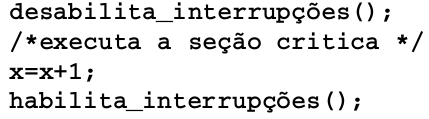
\includegraphics[width=0.5\textwidth]{syscall-inibition}
  \caption{Exemplo de código fonte para acesso à seção crítica, inibindo interrupções}
  \label{fig:syscall-inibition}
\end{figure}

Esta técnica trivialmente \textbf{preserva a exclusão mútua, a espera limitada e o progresso}, dado que apenas um processo apenas executa (e logo acessa a seção crítica) e a tomada da seção crítica é feita de forma direta por cada processo. Porém, por ser uma função crítica, a inibição de interrupções geralmente só pode ser executada pelo SO, sendo \textbf{arriscado disponibilizar este recurso para o usuário}, logo este raramente tem acesso a esta função.

Também é importante notar que esta técnica acaba por ser prejudicada em arquiteturas multiprocessadas: quando um processo inibe as interrupções, ele o faz apenas no seu processador. Logo, processos em outros \textit{cores} que queiram acessar a região crítica poderião fazê-lo sem problema. Logo, esta abordagem é mais interessantes em arquiteturas mono-processadas ou em ambientes protegidos, com pequenas porções de código.





\subsection{Exclusão Mútua com Espera Ocupada}
Também chamada de \textit{busy waiting}, nesta técnica o processo espera a permissão de entrada na seção crítica em um \textit{loop} de teste de permissão, como na Figura \ref{fig:busy-waiting}.

\begin{figure}[ht]
  \centering
  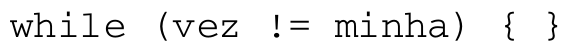
\includegraphics[width=0.5\textwidth]{busy-waiting}
  \caption{Exemplo clássico de \textit{busy waiting}. O processo fica em um \textit{loop} até que a variável \texttt{vez} assuma o valor de \texttt{minha}}
  \label{fig:busy-waiting}
\end{figure}

Esta técnica acaba por disperdiçar muita CPU, uma vez que o processo não é bloqueado e permanece executando, mas de maneira ociosa. Por isso é interessante utilizá-la apenas quando a espera será pequena. Entretanto, em multiprocessadores, isto pode ser interessante, dado que algum outro processo concorrente pode executar na seção crítica durante a espera ociosa.

Dentre as técnicas neste paradigma, a implementação do Algoritmo de Dekker e Peterson não será destrinchada.






\subsubsection{Estrita Alternância}
Nesta técnica, cada processo tem a sua vez de entrar na seção crítica, controlada a partir de uma variável específica para tal, chamada de \textbf{\textit{spin lock}}.

Dessa forma, o processo irá testar a variável, ficando em \textit{busy waiting}, até que ela assuma o valor que sinalize a vez dele executar. Quando o processo terminar a execução, ele dá um outro valor ao \textit{spin lock}.

\begin{figure*}[ht]
  \begin{subfigure}{0.5\textwidth}
    \centering
    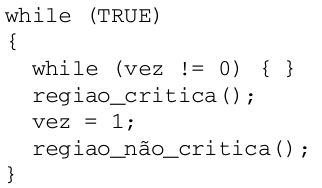
\includegraphics[width=0.9\textwidth]{strict-switch-p1}
    \caption{Código no processo \textbf{\textit{P1}}}
  \end{subfigure}
  ~
  \begin{subfigure}{0.5\textwidth}
    \centering
    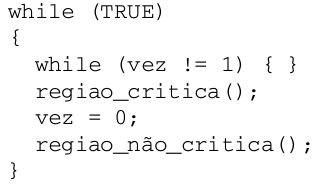
\includegraphics[width=0.9\textwidth]{strict-switch-p2}
    \caption{Código no processo \textbf{\textit{P2}}}
  \end{subfigure}

  \caption{Exemplo clássico de estrita alternância}
  \label{fig:strict-switch}
\end{figure*}

Esta técnica preserva exclusão mútua e a espera limitada. Entretanto, ela \textbf{não preserva o progresso}. Usamos o exemplo da Figura \ref{fig:strict-switch}, dado o caso onde o processo P1 é muito rápido lento que P2. Suponha que P2 está em sua região não-crítica e, nesse meio tempo, P1 executou por inteiro, deixando a variável \texttt{vez} igual a 1. P1 tenta executar o \textit{loop} novamente, mas não irá conseguir até que P2 coloque a variável em 0. Logo, a região crítica está vazia e temos um processo executando fora da região crítica bloqueando um processo que deseja a região.








\subsection{Exclusão Mútua com Bloqueio de Processos}
A outra técnica é o \textbf{bloqueio de processos}, onde o processo que espera a permissão de entrada na seção crítica executa uma primitiva para se bloquear, aguardando até que a seção seja liberada, como na Figura \ref{fig:block-process}.

Esta técnica acaba por \textbf{gerar mais trocas de contextos entre processos, causando esperas longas}.

Existem duas primitivas básicas, as quais, normalmente, envolvem a seção crítica:

\begin{itemize}
  \item Primitiva de \textbf{bloqueio de processo} quando a seção estive ocupada;

  \item Primitiva de \textbf{desbloqueio de processos} à espera da permissão de acesso à seção crítica.
\end{itemize}

\begin{figure}[H]
  \centering
  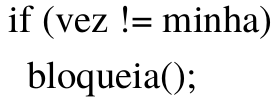
\includegraphics[width=0.35\textwidth]{block-process}
  \caption{Exemplo clássico de bloqueio de processo. O processo checa se as variáveis são iguais e, caso contrário, bloqueia}
  \label{fig:block-process}
\end{figure}




\subsubsection{Semáforos}
Definidos por \textit{Dijkstra} em 1965, consiste em uma variável inteira positiva, que controla o acesso à região crítica, estabelecendo um limite de controle dos sinais de interesse de acesso à ela. O valor inicial do semáforo indica quantos processos podem acessar o recurso simultaneamente, normalmente inicializado com 1.

As operações de manipulação dos semáforos são \textbf{indivisíveis}, ou seja, se um processo está executando-as, ele não pode ser bloqueado. Elas são duas e seu código é mostrado:

\begin{itemize}
  \item \textbf{\textit{Wait} (P ou \textit{down}):} decrementa o valor do semáforo se este for maior que 0. Caso contrário, o processo que executou a operação é bloqueado;

  \item \textbf{\textit{Signal} (V ou \textit{up}):} incremente o valor do semáforo, acordando qualquer processo que esteja bloqueado.
\end{itemize}

\begin{figure*}[ht]

  \begin{subfigure}[t]{.5\textwidth}
    \centering
    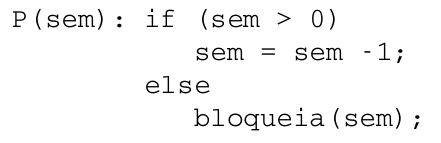
\includegraphics[width=0.9\textwidth]{sem-wait}
    \caption{Operação \textit{Wait}}
    \label{subfig:sem-wait}
  \end{subfigure}
  ~
  \begin{subfigure}[t]{.5\textwidth}
    \centering
    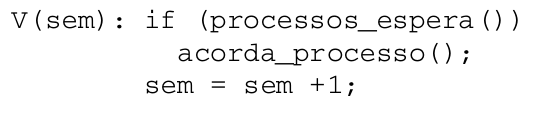
\includegraphics[width=0.9\textwidth]{sem-signal}
    \caption{Operação \textit{Signal}}
    \label{subfig:sem-signal}
  \end{subfigure}

  \caption{Operações de semáforos}
  \label{fig:sem-ops}
\end{figure*}

\textbf{Ideia Geral:} sempre que houver uma região crítica, envolvemos ela com a operação \textit{wait} e \textit{signal}, nesta ordem, como mostra a Figure \ref{fig:semaphore}. Assim, o processo vai checar se o semáforo é maior que 0, ou seja, se a região crítica já está comportando o número limite de processos. Caso esteja, o processo bloqueia, senão, o processo decrementa o valor do semáforo, indicando que há um processo operando ali.
os
Quando o processo acabar de executar a região crítica, ele acorda os outros processos, para que estes possam tentar assumir a região crítica. Finalmente, ele incrementa o semáforo, indicando que há espaço para outro processo acessar o recurso. Note que os outros processos não podem entrar no meio dessas duas ações, pois a ação de \textit{signal} é indivisível.


\begin{figure}[ht]
  \centering
  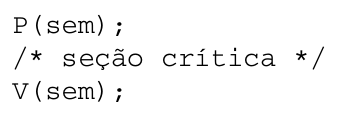
\includegraphics[width=0.35\textwidth]{semaphore}
  \caption{Código de região crítica apropriadamente envolvido por operações de semáforo}
  \label{fig:semaphore}
\end{figure}






\subsubsection{\textit{Locks}}
São estruturas de dados compartilhadas, que garantem a exclusão mútua por \textit{software}, sendo concedido a um processo de cada vez. São operados por duas ações:

\begin{itemize}
  \item \textbf{\textit{Acquire(lock)}:} onde o processo obtém a propriedade do \textit{lock};

  \item \textbf{\textit{Release(lock)}:} onde o processo libera o \textit{lock}.
\end{itemize}

Estas primitivas são chamadas de sistema, podendo ser implementadas tanto como uma espera ocupada ou com bloqueio de processo, sendo este último mais comum e chamado de \textit{mutex}.

\begin{figure}[ht]
  \centering
  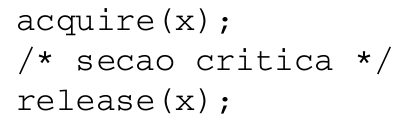
\includegraphics[width=0.35\textwidth]{mutex}
  \caption{Código de região crítica apropriadamente envolvido por operações de \textit{lock}}
  \label{fig:mutex}
\end{figure}


\subsubsection{\textit{Monitores}}
Monitores são conjuntos de procedimentos e dados agrupados em um módulo, indicando que estas entidades são uma região crítica. Estas regiões só podem ser \textbf{acessadas por um processo por vez}, o qual só pode acessar os dados contidos no da seção crítica através de procedimentos definidos pelo monitor. Logo, \textbf{não há acesso direto aos dados por parte do processo requisitante}.

\begin{figure}[ht]
  \centering
  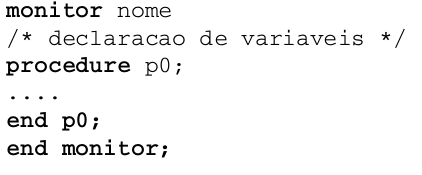
\includegraphics[width=0.55\textwidth]{monitor}
  \caption{Código de região crítica definido dentro de um monitor. Como exemplo, o procedimento \texttt{p0} seria o único com permissão de acessar dados da região crítica}
  \label{fig:monitor}
\end{figure}

O programador é quem definirá as seções críticas, ou seja, o que estará contidos nos monitores. Entretanto, \textbf{a garantia de exclusão mútua é feita pelo compilador}, usando estruturas de baixo nível (como semáforos, por exemplo) e garantindo que apenas um processo acesse o monitor. Por isso, a abstração e \textbf{implementação de monitores deve estar contida na linguagem de programação}, o que raramente é feito.








\subsection{Exemplo Clássico: Produtor-Consumidor}
O problema clássico de Produtor-Consumidor é definido com dois processos \texttt{P0} e \texttt{P1}, que compartilham um \textit{buffer} de tamanho fixo. O processo \texttt{P0} escreve os dados e o processo \texttt{P1} retira-os.

Como o \textit{buffer} tem tamanho fixo, devemos ter uma variável que controle o número de mensagens no mesmo. Assim, o processo produtor não escreve algo quando o \textit{buffer} estiver lotado e o processo consumidor não retira dados quando o \textit{buffer} estiver vazio. Consequentemente, esta variável é compartilhada entre os dois processos, podendo gerar uma condição de corrida.

\begin{figure}[H]
  \centering
  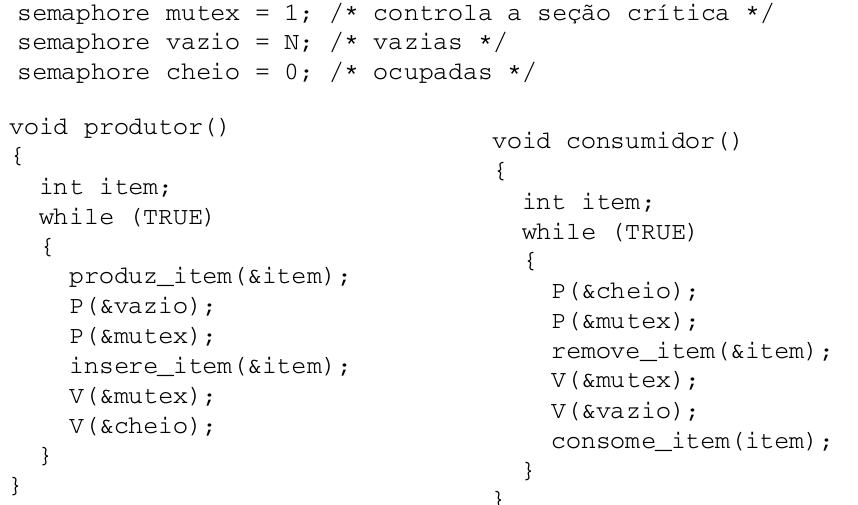
\includegraphics[width=0.75\textwidth]{prod-cons-sem}
  \caption{Solução do problema com semáforos.}
  \label{fig:prod-cons-sem}
\end{figure}

% TODO: colocar o esquema com locks
% \begin{figure}
%   \includegraphics{/path/to/figure}
%   \caption{}
%   \label{}
% \end{figure}

\begin{figure}[H]
  \centering
  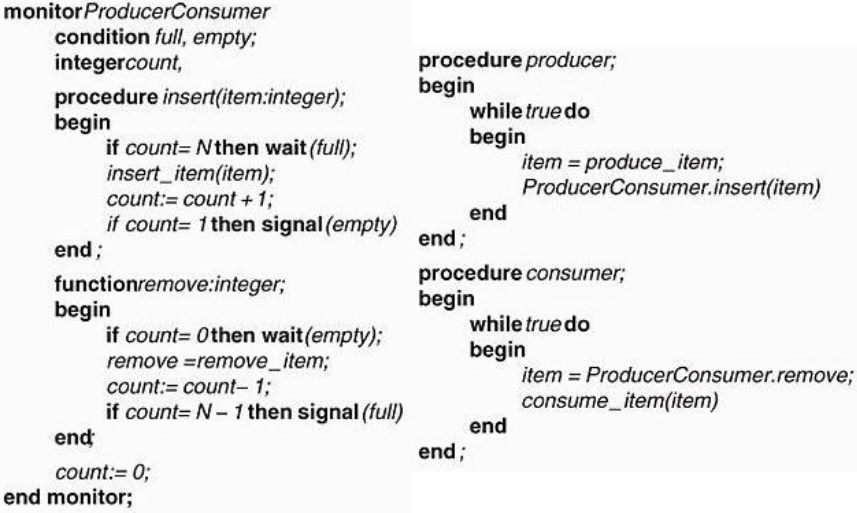
\includegraphics[width=0.85\textwidth]{prod-cons-monitor}
  \caption{Solução do problema com monitores. Definida a variável crítica \texttt{count}, apenas os procedimentos \texttt{insert} e \texttt{remove} podem opera-la. A lógica dos processos são realocadas em procedimentos distintos}
  \label{fig:prod-cons-monitor}
\end{figure}









\section{Troca de Mensagens entre Processos}
Em \textbf{ambientes distribuídos}, onde não há uma memória física compartilhada, as técnicas de compartilhamento de variável acabam por serem ineficazes. Logo, gerou-se a necessidade da troca de mensagens entre os processos para haver a comunicação entre estes. Note que este método pode ser implementado também em ambientes de memória física compartilhada.

A troca de mensagem entre processos é explicita, onde toda comunicação existe no ato de um processo enviar a mensagem e o outro receber. O momento onde a troca ocorre de fato é chamado de \textbf{rendez-vous}. Portanto, há apenas duas primitivas: enviar a mensagem (\textit{send}) e recebê-la (\textit{receive}).

Quando projetamos a comunicação, devemos nos preocupar com alguns aspectos das primitivas. Por exemplo, a cardinalidade: 1 para 1, 1 para $n$ ou $n$ para $n$. Também é importante se preocupar se as primitivas devem ser bloqueadas ou não, ou seja, antes de concluir o \textit{rendez-vouz}, se o processo remetente deve ser bloqueado ou não.

\begin{figure}[h]
  \centering
  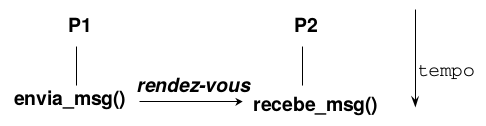
\includegraphics[width=0.7\textwidth]{message-exchange}
  \caption{Ilustração de um \textit{rendez-vouz}}
  \label{fig:rendez-vouz}
\end{figure}

É importante ressaltar que a maioria dos sistemas \textbf{permitem ambas as abordagens de comunicação}, inclusive permitindo o programador misturar primitivas das duas.

\subsection{Primitivas Bloqueadas}
Primitivas bloqueadas ocorrem quando, em um envio de mensagem, o processo remetente é bloqueado até que o \textit{rendez-vouz} aconteça, ou seja, até que o processo destinatário execute a primitiva de recebimento.

Podemos ter dois comportamentos:
\begin{itemize}
  \item \textbf{\textit{Send} antes do \textit{Receive}:} primeiro, o processo remetente envia a mensagem e se bloqueia, aguardando o \textit{rendez-vouz}. O processo destinatário se bloqueia apenas para receber a mensagem, desbloqueando logo depois. \textbf{O maior tempo de bloqueio está do lado do remetente};

  \item \textbf{\textit{Receive} antes do \textit{Send}:} primeiro, o processo destinatário se bloqueia, aguardando a mensagem, desbloqueando apenas quando recebe. O processo remetente se bloqueia apenas no momento do envio da mensagem e logo recomeça a execução. \textbf{O maior tempo de bloqueio está do lado do destinatário}.
\end{itemize}

\begin{figure*}[ht]
  \begin{subfigure}[t]{0.5\textwidth}
    \centering
    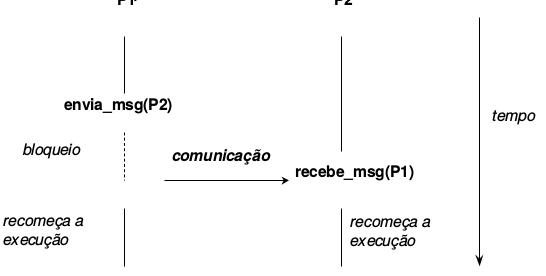
\includegraphics[width=0.85\textwidth]{block-send-receive}
    \caption{\textit{Send} antes do \textit{receive}}
    \label{subfig:block-send-receive}
  \end{subfigure}
  ~
  \begin{subfigure}[t]{0.5\textwidth}
    \centering
    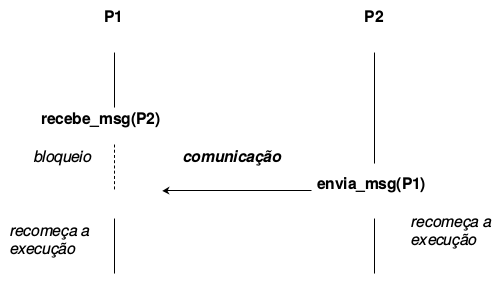
\includegraphics[width=0.85\textwidth]{block-receive-send}
    \caption{\textit{Receive} antes do \textit{send}}
    \label{subfig:block-receive-send}
  \end{subfigure}

  \caption{Tipos de comportamento para primitivas blocantes}
  \label{fig:blocking-types}
\end{figure*}

Dizemos que essa é uma \textbf{comunicação síncrona}, dado que no memento da troca de mensagens, cada processo envolvido na comunicação sabe exatamente o estado do outro, pois ambos estão executando a primitiva de comunicação. Logo, implicitamente os processos também estão comunicando os seus estados de execução. Como vantagem, estas primitivas \textbf{tem implementação mais simples}.

Quando dois processos executam um \textit{receive}, esperando um mensagem do outro, ambos se encontram bloqueados e aguardando um recurso do outro. Logo, vemos a \textbf{possibilidade de \textit{deadlock}} nesta comunicação. Tal situação pode ser resolvida com a temporização da primitiva de \textit{receive}, estabelecendo um tempo máximo que o processo pode ficar bloqueado.

\begin{figure*}[ht]
  \begin{subfigure}[t]{0.5\textwidth}
    \centering
    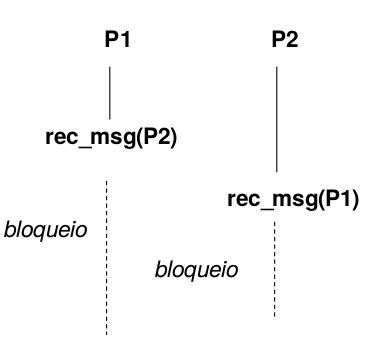
\includegraphics[width=0.7\textwidth]{block-deadlock}
    \caption{Possível \textit{deadlock}}
    \label{subfig:block-deadlock}
  \end{subfigure}
  ~
  \begin{subfigure}[t]{0.5\textwidth}
    \centering
    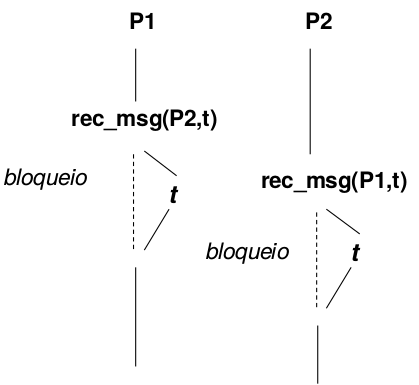
\includegraphics[width=0.7\textwidth]{block-temporizer}
    \caption{Solução com temporizadores}
    \label{subfig:block-temporizer}
  \end{subfigure}

  \caption{Possível desvantagem ao utilizar primitivas blocantes}
  \label{fig:block-deadlock-scheme}
\end{figure*}

Outra desvantagem é a \textbf{perda de paralelismo}, causada pela primitiva blocante. Um contorno para este problema é a utilização de \textit{threads} para realizar as primitivas, o que é chamado de \textbf{comunicação pseudo-assíncrona}. Tal abordagem está sendo muito estudada por juntar o melhor dos mundos das abordagens síncronas e assíncronas.

\begin{figure*}[ht]
  \begin{subfigure}[t]{0.5\textwidth}
    \centering
    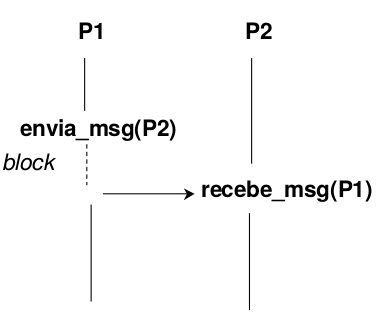
\includegraphics[width=0.7\textwidth]{block-blocking}
    \caption{Problema de perda de paralelismo}
    \label{subfig:block-pseudo-async1}
  \end{subfigure}
  ~
  \begin{subfigure}[t]{0.5\textwidth}
    \centering
    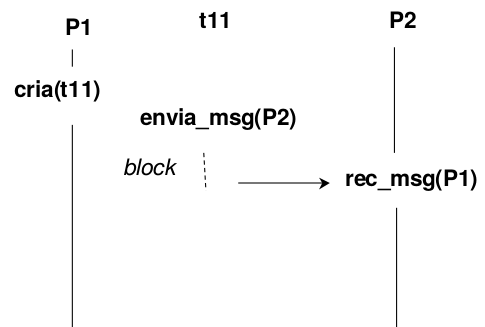
\includegraphics[width=0.7\textwidth]{block-pseudo-async}
    \caption{Solução com \textit{thread}}
    \label{subfig:block-pseudo-async2}
  \end{subfigure}

  \caption{Problema e solução com primitivas pseudo-assíncronas}
  \label{fig:block-pseudo-async}
\end{figure*}


\subsection{Primitivas Não-Bloqueadas}
Aqui, tanto o processo remetente como o destinatário não são bloqueados ao realizar as primitivas. Logo, esta técnica \textbf{oferece um alto grau de concorrência}.

Assim como nas síncronas, temos dois comportamentos. Quando o \textit{send} vem antes do \textit{receive}, o remetente simplesmente envia a mensagem, sem bloquear, e o remetente recebe a mesma, ambos usando as primitivas padrões.

\begin{figure}[ht]
  \centering
  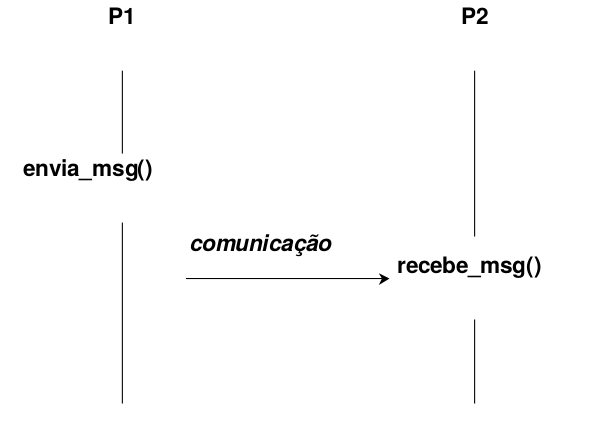
\includegraphics[width=0.5\textwidth]{nonblock-sendreceive}
  \caption{\textit{Send} antes de \textit{receive} em primitivas não-blocantes}
  \label{fig:nonblock-sendreceive}
\end{figure}

Entretanto, como o \textit{receive} não é blocante, na estratégia de \textit{receive} antes do \textit{send} é capaz que a mensagem esperada do remetente ainda não tenha chegado. Para isso, existem duas abordagens:

\begin{itemize}
  \item \textbf{NOMSG:} ao constatar o não recebimento da mensagem, a primitiva retorna um sinal de \textit{mensagem não recebida} (\texttt{NOMSG}) para o processo;

  \item \textbf{\textit{Probing}:} ao constatar o não recebimento da mensagem, é feita uma primitiva que requisita a mensagem ao remetente. Em certas situações, essa primitiva pode acarretar no bloqueio do destinatário (note que ela não é um \textit{send} ou \textit{receive}).
\end{itemize}

\begin{figure*}[ht]
  \begin{subfigure}{0.5\textwidth}
    \centering
    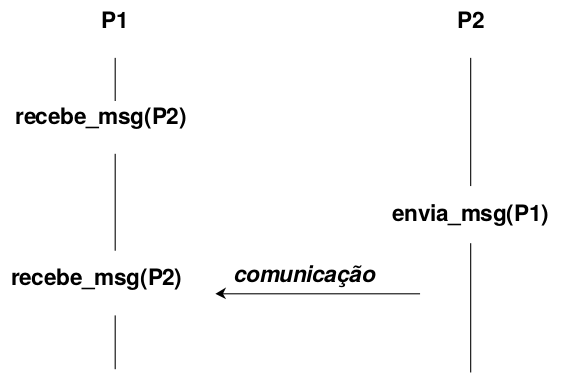
\includegraphics[width=0.7\textwidth]{nonblock-nomsg}
    \caption{Abordagem com \texttt{NOMSG}}
    \label{subfig:nonblock-nomsg}
  \end{subfigure}
  ~
  \begin{subfigure}{0.5\textwidth}
    \centering
    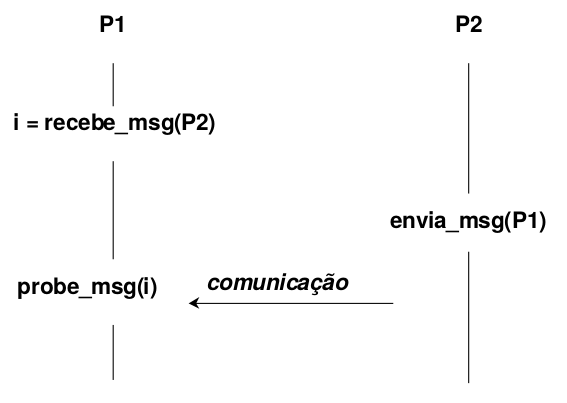
\includegraphics[width=0.7\textwidth]{nonblock-probing}
    \caption{Abordagem com \textit{probing}}
    \label{subfig:nonblock-probing}
  \end{subfigure}

  \caption{Comportamentos para \textit{receive} antes de \textit{send} em primitivas não-blocantes}
  \label{fig:messages-nonblock}
\end{figure*}
